% Created by tikzDevice version 0.12 on 2019-04-10 00:21:38
% !TEX encoding = UTF-8 Unicode
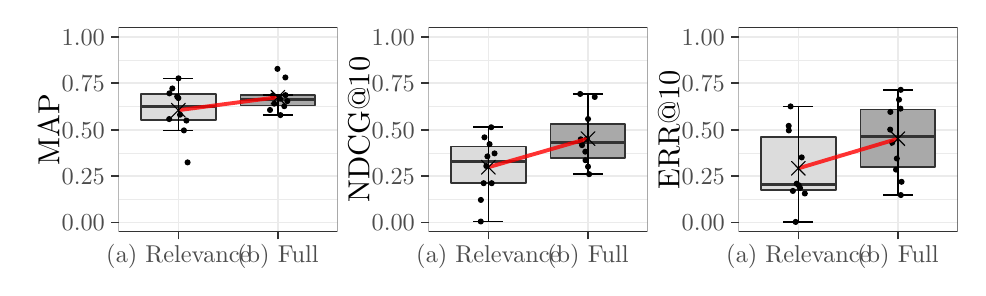
\begin{tikzpicture}[x=1pt,y=1pt]
\definecolor{fillColor}{RGB}{255,255,255}
\path[use as bounding box,fill=fillColor,fill opacity=0.00] (0,0) rectangle (336.06, 86.72);
\begin{scope}
\path[clip] (  0.00,  0.00) rectangle (112.02, 86.72);
\definecolor{drawColor}{RGB}{255,255,255}
\definecolor{fillColor}{RGB}{255,255,255}

\path[draw=drawColor,line width= 0.6pt,line join=round,line cap=round,fill=fillColor] ( -0.00,  0.00) rectangle (112.02, 86.72);
\end{scope}
\begin{scope}
\path[clip] ( 32.86, 12.95) rectangle (112.02, 86.72);
\definecolor{fillColor}{RGB}{255,255,255}

\path[fill=fillColor] ( 32.86, 12.95) rectangle (112.02, 86.72);
\definecolor{drawColor}{gray}{0.92}

\path[draw=drawColor,line width= 0.3pt,line join=round] ( 32.86, 24.69) --
	(112.02, 24.69);

\path[draw=drawColor,line width= 0.3pt,line join=round] ( 32.86, 41.46) --
	(112.02, 41.46);

\path[draw=drawColor,line width= 0.3pt,line join=round] ( 32.86, 58.22) --
	(112.02, 58.22);

\path[draw=drawColor,line width= 0.3pt,line join=round] ( 32.86, 74.99) --
	(112.02, 74.99);

\path[draw=drawColor,line width= 0.6pt,line join=round] ( 32.86, 16.31) --
	(112.02, 16.31);

\path[draw=drawColor,line width= 0.6pt,line join=round] ( 32.86, 33.07) --
	(112.02, 33.07);

\path[draw=drawColor,line width= 0.6pt,line join=round] ( 32.86, 49.84) --
	(112.02, 49.84);

\path[draw=drawColor,line width= 0.6pt,line join=round] ( 32.86, 66.61) --
	(112.02, 66.61);

\path[draw=drawColor,line width= 0.6pt,line join=round] ( 32.86, 83.37) --
	(112.02, 83.37);

\path[draw=drawColor,line width= 0.6pt,line join=round] ( 54.45, 12.95) --
	( 54.45, 86.72);

\path[draw=drawColor,line width= 0.6pt,line join=round] ( 90.43, 12.95) --
	( 90.43, 86.72);

\path[] ( 52.49, 36.08) -- ( 56.41, 40.01);

\path[] ( 52.49, 40.01) -- ( 56.41, 36.08);
\definecolor{drawColor}{gray}{0.20}

\path[draw=drawColor,line width= 0.6pt,line join=round] ( 54.45, 62.69) -- ( 54.45, 68.41);

\path[draw=drawColor,line width= 0.6pt,line join=round] ( 54.45, 53.29) -- ( 54.45, 49.60);
\definecolor{fillColor}{RGB}{220,220,220}

\path[draw=drawColor,line width= 0.6pt,line join=round,line cap=round,fill=fillColor] ( 40.96, 62.69) --
	( 40.96, 53.29) --
	( 67.94, 53.29) --
	( 67.94, 62.69) --
	( 40.96, 62.69) --
	cycle;

\path[draw=drawColor,line width= 1.1pt,line join=round] ( 40.96, 58.28) -- ( 67.94, 58.28);

\path[] ( 88.47, 66.77) -- ( 92.39, 70.69);

\path[] ( 88.47, 70.69) -- ( 92.39, 66.77);

\path[] ( 88.47, 69.87) -- ( 92.39, 73.79);

\path[] ( 88.47, 73.79) -- ( 92.39, 69.87);

\path[draw=drawColor,line width= 0.6pt,line join=round] ( 90.43, 62.32) -- ( 90.43, 62.34);

\path[draw=drawColor,line width= 0.6pt,line join=round] ( 90.43, 58.57) -- ( 90.43, 55.13);
\definecolor{fillColor}{RGB}{169,169,169}

\path[draw=drawColor,line width= 0.6pt,line join=round,line cap=round,fill=fillColor] ( 76.94, 62.32) --
	( 76.94, 58.57) --
	(103.92, 58.57) --
	(103.92, 62.32) --
	( 76.94, 62.32) --
	cycle;

\path[draw=drawColor,line width= 1.1pt,line join=round] ( 76.94, 60.61) -- (103.92, 60.61);
\definecolor{drawColor}{RGB}{0,0,0}
\definecolor{fillColor}{RGB}{0,0,0}

\path[draw=drawColor,line width= 0.4pt,line join=round,line cap=round,fill=fillColor] ( 52.27, 64.75) circle (  0.89);

\path[draw=drawColor,line width= 0.4pt,line join=round,line cap=round,fill=fillColor] ( 54.45, 61.28) circle (  0.89);

\path[draw=drawColor,line width= 0.4pt,line join=round,line cap=round,fill=fillColor] ( 54.03, 61.82) circle (  0.89);

\path[draw=drawColor,line width= 0.4pt,line join=round,line cap=round,fill=fillColor] ( 56.46, 49.60) circle (  0.89);

\path[draw=drawColor,line width= 0.4pt,line join=round,line cap=round,fill=fillColor] ( 57.36, 53.16) circle (  0.89);

\path[draw=drawColor,line width= 0.4pt,line join=round,line cap=round,fill=fillColor] ( 54.49, 68.41) circle (  0.89);

\path[draw=drawColor,line width= 0.4pt,line join=round,line cap=round,fill=fillColor] ( 51.14, 53.69) circle (  0.89);

\path[draw=drawColor,line width= 0.4pt,line join=round,line cap=round,fill=fillColor] ( 57.78, 38.04) circle (  0.89);

\path[draw=drawColor,line width= 0.4pt,line join=round,line cap=round,fill=fillColor] ( 51.22, 62.98) circle (  0.89);

\path[draw=drawColor,line width= 0.4pt,line join=round,line cap=round,fill=fillColor] ( 55.06, 55.28) circle (  0.89);

\path[draw=drawColor,line width= 0.4pt,line join=round,line cap=round,fill=fillColor] ( 89.10, 59.25) circle (  0.89);

\path[draw=drawColor,line width= 0.4pt,line join=round,line cap=round,fill=fillColor] ( 92.72, 58.35) circle (  0.89);

\path[draw=drawColor,line width= 0.4pt,line join=round,line cap=round,fill=fillColor] ( 91.32, 55.13) circle (  0.89);

\path[draw=drawColor,line width= 0.4pt,line join=round,line cap=round,fill=fillColor] ( 91.20, 61.03) circle (  0.89);

\path[draw=drawColor,line width= 0.4pt,line join=round,line cap=round,fill=fillColor] ( 93.12, 68.73) circle (  0.89);

\path[draw=drawColor,line width= 0.4pt,line join=round,line cap=round,fill=fillColor] ( 93.16, 62.34) circle (  0.89);

\path[draw=drawColor,line width= 0.4pt,line join=round,line cap=round,fill=fillColor] ( 87.57, 56.98) circle (  0.89);

\path[draw=drawColor,line width= 0.4pt,line join=round,line cap=round,fill=fillColor] ( 90.26, 71.83) circle (  0.89);

\path[draw=drawColor,line width= 0.4pt,line join=round,line cap=round,fill=fillColor] ( 88.60, 62.26) circle (  0.89);

\path[draw=drawColor,line width= 0.4pt,line join=round,line cap=round,fill=fillColor] ( 93.82, 60.19) circle (  0.89);
\definecolor{drawColor}{RGB}{255,0,0}

\path[draw=drawColor,draw opacity=0.80,line width= 1.4pt,line join=round] ( 54.45, 56.90) --
	( 90.43, 61.61);
\definecolor{drawColor}{RGB}{0,0,0}

\path[draw=drawColor,line width= 0.4pt,line join=round,line cap=round] ( 51.95, 54.40) -- ( 56.95, 59.40);

\path[draw=drawColor,line width= 0.4pt,line join=round,line cap=round] ( 51.95, 59.40) -- ( 56.95, 54.40);

\path[draw=drawColor,line width= 0.4pt,line join=round,line cap=round] ( 87.93, 59.11) -- ( 92.93, 64.11);

\path[draw=drawColor,line width= 0.4pt,line join=round,line cap=round] ( 87.93, 64.11) -- ( 92.93, 59.11);

\path[draw=drawColor,line width= 0.6pt,line join=round] ( 49.05, 68.41) --
	( 59.85, 68.41);

\path[draw=drawColor,line width= 0.6pt,line join=round] ( 54.45, 68.41) --
	( 54.45, 49.60);

\path[draw=drawColor,line width= 0.6pt,line join=round] ( 49.05, 49.60) --
	( 59.85, 49.60);

\path[draw=drawColor,line width= 0.6pt,line join=round] ( 85.03, 62.34) --
	( 95.83, 62.34);

\path[draw=drawColor,line width= 0.6pt,line join=round] ( 90.43, 62.34) --
	( 90.43, 55.13);

\path[draw=drawColor,line width= 0.6pt,line join=round] ( 85.03, 55.13) --
	( 95.83, 55.13);
\definecolor{drawColor}{gray}{0.20}

\path[draw=drawColor,line width= 0.6pt,line join=round,line cap=round] ( 32.86, 12.95) rectangle (112.02, 86.72);
\end{scope}
\begin{scope}
\path[clip] (  0.00,  0.00) rectangle (336.06, 86.72);
\definecolor{drawColor}{gray}{0.30}

\node[text=drawColor,anchor=base east,inner sep=0pt, outer sep=0pt, scale=  0.88] at ( 27.91, 13.28) {0.00};

\node[text=drawColor,anchor=base east,inner sep=0pt, outer sep=0pt, scale=  0.88] at ( 27.91, 30.04) {0.25};

\node[text=drawColor,anchor=base east,inner sep=0pt, outer sep=0pt, scale=  0.88] at ( 27.91, 46.81) {0.50};

\node[text=drawColor,anchor=base east,inner sep=0pt, outer sep=0pt, scale=  0.88] at ( 27.91, 63.57) {0.75};

\node[text=drawColor,anchor=base east,inner sep=0pt, outer sep=0pt, scale=  0.88] at ( 27.91, 80.34) {1.00};
\end{scope}
\begin{scope}
\path[clip] (  0.00,  0.00) rectangle (336.06, 86.72);
\definecolor{drawColor}{gray}{0.20}

\path[draw=drawColor,line width= 0.6pt,line join=round] ( 30.11, 16.31) --
	( 32.86, 16.31);

\path[draw=drawColor,line width= 0.6pt,line join=round] ( 30.11, 33.07) --
	( 32.86, 33.07);

\path[draw=drawColor,line width= 0.6pt,line join=round] ( 30.11, 49.84) --
	( 32.86, 49.84);

\path[draw=drawColor,line width= 0.6pt,line join=round] ( 30.11, 66.61) --
	( 32.86, 66.61);

\path[draw=drawColor,line width= 0.6pt,line join=round] ( 30.11, 83.37) --
	( 32.86, 83.37);
\end{scope}
\begin{scope}
\path[clip] (  0.00,  0.00) rectangle (336.06, 86.72);
\definecolor{drawColor}{gray}{0.20}

\path[draw=drawColor,line width= 0.6pt,line join=round] ( 54.45, 10.20) --
	( 54.45, 12.95);

\path[draw=drawColor,line width= 0.6pt,line join=round] ( 90.43, 10.20) --
	( 90.43, 12.95);
\end{scope}
\begin{scope}
\path[clip] (  0.00,  0.00) rectangle (336.06, 86.72);
\definecolor{drawColor}{gray}{0.30}

\node[text=drawColor,anchor=base,inner sep=0pt, outer sep=0pt, scale=  0.88] at ( 54.45,  1.94) {(a) Relevance};

\node[text=drawColor,anchor=base,inner sep=0pt, outer sep=0pt, scale=  0.88] at ( 90.43,  1.94) {(b) Full};
\end{scope}
\begin{scope}
\path[clip] (  0.00,  0.00) rectangle (336.06, 86.72);
\definecolor{drawColor}{RGB}{0,0,0}

\node[text=drawColor,rotate= 90.00,anchor=base,inner sep=0pt, outer sep=0pt, scale=  1.10] at ( 11.46, 49.84) {MAP};
\end{scope}
\begin{scope}
\path[clip] (112.02,  0.00) rectangle (224.04, 86.72);
\definecolor{drawColor}{RGB}{255,255,255}
\definecolor{fillColor}{RGB}{255,255,255}

\path[draw=drawColor,line width= 0.6pt,line join=round,line cap=round,fill=fillColor] (112.02,  0.00) rectangle (224.04, 86.72);
\end{scope}
\begin{scope}
\path[clip] (144.88, 12.95) rectangle (224.04, 86.72);
\definecolor{fillColor}{RGB}{255,255,255}

\path[fill=fillColor] (144.88, 12.95) rectangle (224.04, 86.72);
\definecolor{drawColor}{gray}{0.92}

\path[draw=drawColor,line width= 0.3pt,line join=round] (144.88, 24.69) --
	(224.04, 24.69);

\path[draw=drawColor,line width= 0.3pt,line join=round] (144.88, 41.46) --
	(224.04, 41.46);

\path[draw=drawColor,line width= 0.3pt,line join=round] (144.88, 58.22) --
	(224.04, 58.22);

\path[draw=drawColor,line width= 0.3pt,line join=round] (144.88, 74.99) --
	(224.04, 74.99);

\path[draw=drawColor,line width= 0.6pt,line join=round] (144.88, 16.31) --
	(224.04, 16.31);

\path[draw=drawColor,line width= 0.6pt,line join=round] (144.88, 33.07) --
	(224.04, 33.07);

\path[draw=drawColor,line width= 0.6pt,line join=round] (144.88, 49.84) --
	(224.04, 49.84);

\path[draw=drawColor,line width= 0.6pt,line join=round] (144.88, 66.61) --
	(224.04, 66.61);

\path[draw=drawColor,line width= 0.6pt,line join=round] (144.88, 83.37) --
	(224.04, 83.37);

\path[draw=drawColor,line width= 0.6pt,line join=round] (166.47, 12.95) --
	(166.47, 86.72);

\path[draw=drawColor,line width= 0.6pt,line join=round] (202.45, 12.95) --
	(202.45, 86.72);
\definecolor{drawColor}{gray}{0.20}

\path[draw=drawColor,line width= 0.6pt,line join=round] (166.47, 43.79) -- (166.47, 50.74);

\path[draw=drawColor,line width= 0.6pt,line join=round] (166.47, 30.52) -- (166.47, 16.68);
\definecolor{fillColor}{RGB}{220,220,220}

\path[draw=drawColor,line width= 0.6pt,line join=round,line cap=round,fill=fillColor] (152.97, 43.79) --
	(152.97, 30.52) --
	(179.96, 30.52) --
	(179.96, 43.79) --
	(152.97, 43.79) --
	cycle;

\path[draw=drawColor,line width= 1.1pt,line join=round] (152.97, 38.47) -- (179.96, 38.47);

\path[draw=drawColor,line width= 0.6pt,line join=round] (202.45, 51.93) -- (202.45, 62.77);

\path[draw=drawColor,line width= 0.6pt,line join=round] (202.45, 39.59) -- (202.45, 33.78);
\definecolor{fillColor}{RGB}{169,169,169}

\path[draw=drawColor,line width= 0.6pt,line join=round,line cap=round,fill=fillColor] (188.96, 51.93) --
	(188.96, 39.59) --
	(215.94, 39.59) --
	(215.94, 51.93) --
	(188.96, 51.93) --
	cycle;

\path[draw=drawColor,line width= 1.1pt,line join=round] (188.96, 45.32) -- (215.94, 45.32);
\definecolor{drawColor}{RGB}{0,0,0}
\definecolor{fillColor}{RGB}{0,0,0}

\path[draw=drawColor,line width= 0.4pt,line join=round,line cap=round,fill=fillColor] (166.12, 40.20) circle (  0.89);

\path[draw=drawColor,line width= 0.4pt,line join=round,line cap=round,fill=fillColor] (165.06, 47.10) circle (  0.89);

\path[draw=drawColor,line width= 0.4pt,line join=round,line cap=round,fill=fillColor] (166.90, 44.63) circle (  0.89);

\path[draw=drawColor,line width= 0.4pt,line join=round,line cap=round,fill=fillColor] (167.68, 30.52) circle (  0.89);

\path[draw=drawColor,line width= 0.4pt,line join=round,line cap=round,fill=fillColor] (163.76, 24.48) circle (  0.89);

\path[draw=drawColor,line width= 0.4pt,line join=round,line cap=round,fill=fillColor] (168.70, 41.29) circle (  0.89);

\path[draw=drawColor,line width= 0.4pt,line join=round,line cap=round,fill=fillColor] (164.78, 30.52) circle (  0.89);

\path[draw=drawColor,line width= 0.4pt,line join=round,line cap=round,fill=fillColor] (163.73, 16.68) circle (  0.89);

\path[draw=drawColor,line width= 0.4pt,line join=round,line cap=round,fill=fillColor] (167.50, 50.74) circle (  0.89);

\path[draw=drawColor,line width= 0.4pt,line join=round,line cap=round,fill=fillColor] (165.73, 36.73) circle (  0.89);

\path[draw=drawColor,line width= 0.4pt,line join=round,line cap=round,fill=fillColor] (201.56, 38.81) circle (  0.89);

\path[draw=drawColor,line width= 0.4pt,line join=round,line cap=round,fill=fillColor] (204.91, 61.68) circle (  0.89);

\path[draw=drawColor,line width= 0.4pt,line join=round,line cap=round,fill=fillColor] (201.50, 41.91) circle (  0.89);

\path[draw=drawColor,line width= 0.4pt,line join=round,line cap=round,fill=fillColor] (199.65, 62.77) circle (  0.89);

\path[draw=drawColor,line width= 0.4pt,line join=round,line cap=round,fill=fillColor] (202.48, 36.49) circle (  0.89);

\path[draw=drawColor,line width= 0.4pt,line join=round,line cap=round,fill=fillColor] (202.89, 33.78) circle (  0.89);

\path[draw=drawColor,line width= 0.4pt,line join=round,line cap=round,fill=fillColor] (202.49, 53.72) circle (  0.89);

\path[draw=drawColor,line width= 0.4pt,line join=round,line cap=round,fill=fillColor] (200.31, 44.27) circle (  0.89);

\path[draw=drawColor,line width= 0.4pt,line join=round,line cap=round,fill=fillColor] (202.07, 46.54) circle (  0.89);

\path[draw=drawColor,line width= 0.4pt,line join=round,line cap=round,fill=fillColor] (199.85, 46.37) circle (  0.89);
\definecolor{drawColor}{RGB}{255,0,0}

\path[draw=drawColor,draw opacity=0.80,line width= 1.4pt,line join=round] (166.47, 36.29) --
	(202.45, 46.64);
\definecolor{drawColor}{RGB}{0,0,0}

\path[draw=drawColor,line width= 0.4pt,line join=round,line cap=round] (163.97, 33.79) -- (168.97, 38.79);

\path[draw=drawColor,line width= 0.4pt,line join=round,line cap=round] (163.97, 38.79) -- (168.97, 33.79);

\path[draw=drawColor,line width= 0.4pt,line join=round,line cap=round] (199.95, 44.14) -- (204.95, 49.13);

\path[draw=drawColor,line width= 0.4pt,line join=round,line cap=round] (199.95, 49.13) -- (204.95, 44.14);

\path[draw=drawColor,line width= 0.6pt,line join=round] (161.07, 50.74) --
	(171.86, 50.74);

\path[draw=drawColor,line width= 0.6pt,line join=round] (166.47, 50.74) --
	(166.47, 16.68);

\path[draw=drawColor,line width= 0.6pt,line join=round] (161.07, 16.68) --
	(171.86, 16.68);

\path[draw=drawColor,line width= 0.6pt,line join=round] (197.05, 62.77) --
	(207.85, 62.77);

\path[draw=drawColor,line width= 0.6pt,line join=round] (202.45, 62.77) --
	(202.45, 33.78);

\path[draw=drawColor,line width= 0.6pt,line join=round] (197.05, 33.78) --
	(207.85, 33.78);
\definecolor{drawColor}{gray}{0.20}

\path[draw=drawColor,line width= 0.6pt,line join=round,line cap=round] (144.88, 12.95) rectangle (224.04, 86.72);
\end{scope}
\begin{scope}
\path[clip] (  0.00,  0.00) rectangle (336.06, 86.72);
\definecolor{drawColor}{gray}{0.30}

\node[text=drawColor,anchor=base east,inner sep=0pt, outer sep=0pt, scale=  0.88] at (139.93, 13.28) {0.00};

\node[text=drawColor,anchor=base east,inner sep=0pt, outer sep=0pt, scale=  0.88] at (139.93, 30.04) {0.25};

\node[text=drawColor,anchor=base east,inner sep=0pt, outer sep=0pt, scale=  0.88] at (139.93, 46.81) {0.50};

\node[text=drawColor,anchor=base east,inner sep=0pt, outer sep=0pt, scale=  0.88] at (139.93, 63.57) {0.75};

\node[text=drawColor,anchor=base east,inner sep=0pt, outer sep=0pt, scale=  0.88] at (139.93, 80.34) {1.00};
\end{scope}
\begin{scope}
\path[clip] (  0.00,  0.00) rectangle (336.06, 86.72);
\definecolor{drawColor}{gray}{0.20}

\path[draw=drawColor,line width= 0.6pt,line join=round] (142.13, 16.31) --
	(144.88, 16.31);

\path[draw=drawColor,line width= 0.6pt,line join=round] (142.13, 33.07) --
	(144.88, 33.07);

\path[draw=drawColor,line width= 0.6pt,line join=round] (142.13, 49.84) --
	(144.88, 49.84);

\path[draw=drawColor,line width= 0.6pt,line join=round] (142.13, 66.61) --
	(144.88, 66.61);

\path[draw=drawColor,line width= 0.6pt,line join=round] (142.13, 83.37) --
	(144.88, 83.37);
\end{scope}
\begin{scope}
\path[clip] (  0.00,  0.00) rectangle (336.06, 86.72);
\definecolor{drawColor}{gray}{0.20}

\path[draw=drawColor,line width= 0.6pt,line join=round] (166.47, 10.20) --
	(166.47, 12.95);

\path[draw=drawColor,line width= 0.6pt,line join=round] (202.45, 10.20) --
	(202.45, 12.95);
\end{scope}
\begin{scope}
\path[clip] (  0.00,  0.00) rectangle (336.06, 86.72);
\definecolor{drawColor}{gray}{0.30}

\node[text=drawColor,anchor=base,inner sep=0pt, outer sep=0pt, scale=  0.88] at (166.47,  1.94) {(a) Relevance};

\node[text=drawColor,anchor=base,inner sep=0pt, outer sep=0pt, scale=  0.88] at (202.45,  1.94) {(b) Full};
\end{scope}
\begin{scope}
\path[clip] (  0.00,  0.00) rectangle (336.06, 86.72);
\definecolor{drawColor}{RGB}{0,0,0}

\node[text=drawColor,rotate= 90.00,anchor=base,inner sep=0pt, outer sep=0pt, scale=  1.10] at (123.48, 49.84) {NDCG@10};
\end{scope}
\begin{scope}
\path[clip] (224.04,  0.00) rectangle (336.06, 86.72);
\definecolor{drawColor}{RGB}{255,255,255}
\definecolor{fillColor}{RGB}{255,255,255}

\path[draw=drawColor,line width= 0.6pt,line join=round,line cap=round,fill=fillColor] (224.04,  0.00) rectangle (336.06, 86.72);
\end{scope}
\begin{scope}
\path[clip] (256.90, 12.95) rectangle (336.06, 86.72);
\definecolor{fillColor}{RGB}{255,255,255}

\path[fill=fillColor] (256.90, 12.95) rectangle (336.06, 86.72);
\definecolor{drawColor}{gray}{0.92}

\path[draw=drawColor,line width= 0.3pt,line join=round] (256.90, 24.69) --
	(336.06, 24.69);

\path[draw=drawColor,line width= 0.3pt,line join=round] (256.90, 41.46) --
	(336.06, 41.46);

\path[draw=drawColor,line width= 0.3pt,line join=round] (256.90, 58.22) --
	(336.06, 58.22);

\path[draw=drawColor,line width= 0.3pt,line join=round] (256.90, 74.99) --
	(336.06, 74.99);

\path[draw=drawColor,line width= 0.6pt,line join=round] (256.90, 16.31) --
	(336.06, 16.31);

\path[draw=drawColor,line width= 0.6pt,line join=round] (256.90, 33.07) --
	(336.06, 33.07);

\path[draw=drawColor,line width= 0.6pt,line join=round] (256.90, 49.84) --
	(336.06, 49.84);

\path[draw=drawColor,line width= 0.6pt,line join=round] (256.90, 66.61) --
	(336.06, 66.61);

\path[draw=drawColor,line width= 0.6pt,line join=round] (256.90, 83.37) --
	(336.06, 83.37);

\path[draw=drawColor,line width= 0.6pt,line join=round] (278.49, 12.95) --
	(278.49, 86.72);

\path[draw=drawColor,line width= 0.6pt,line join=round] (314.47, 12.95) --
	(314.47, 86.72);
\definecolor{drawColor}{gray}{0.20}

\path[draw=drawColor,line width= 0.6pt,line join=round] (278.49, 47.16) -- (278.49, 58.27);

\path[draw=drawColor,line width= 0.6pt,line join=round] (278.49, 27.99) -- (278.49, 16.52);
\definecolor{fillColor}{RGB}{220,220,220}

\path[draw=drawColor,line width= 0.6pt,line join=round,line cap=round,fill=fillColor] (264.99, 47.16) --
	(264.99, 27.99) --
	(291.98, 27.99) --
	(291.98, 47.16) --
	(264.99, 47.16) --
	cycle;

\path[draw=drawColor,line width= 1.1pt,line join=round] (264.99, 30.06) -- (291.98, 30.06);

\path[draw=drawColor,line width= 0.6pt,line join=round] (314.47, 57.17) -- (314.47, 64.26);

\path[draw=drawColor,line width= 0.6pt,line join=round] (314.47, 36.44) -- (314.47, 26.23);
\definecolor{fillColor}{RGB}{169,169,169}

\path[draw=drawColor,line width= 0.6pt,line join=round,line cap=round,fill=fillColor] (300.97, 57.17) --
	(300.97, 36.44) --
	(327.96, 36.44) --
	(327.96, 57.17) --
	(300.97, 57.17) --
	cycle;

\path[draw=drawColor,line width= 1.1pt,line join=round] (300.97, 47.54) -- (327.96, 47.54);
\definecolor{drawColor}{RGB}{0,0,0}
\definecolor{fillColor}{RGB}{0,0,0}

\path[draw=drawColor,line width= 0.4pt,line join=round,line cap=round,fill=fillColor] (279.09, 28.77) circle (  0.89);

\path[draw=drawColor,line width= 0.4pt,line join=round,line cap=round,fill=fillColor] (275.03, 49.59) circle (  0.89);

\path[draw=drawColor,line width= 0.4pt,line join=round,line cap=round,fill=fillColor] (275.00, 51.24) circle (  0.89);

\path[draw=drawColor,line width= 0.4pt,line join=round,line cap=round,fill=fillColor] (278.62, 29.77) circle (  0.89);

\path[draw=drawColor,line width= 0.4pt,line join=round,line cap=round,fill=fillColor] (280.82, 26.80) circle (  0.89);

\path[draw=drawColor,line width= 0.4pt,line join=round,line cap=round,fill=fillColor] (277.87, 30.35) circle (  0.89);

\path[draw=drawColor,line width= 0.4pt,line join=round,line cap=round,fill=fillColor] (276.50, 27.73) circle (  0.89);

\path[draw=drawColor,line width= 0.4pt,line join=round,line cap=round,fill=fillColor] (277.50, 16.52) circle (  0.89);

\path[draw=drawColor,line width= 0.4pt,line join=round,line cap=round,fill=fillColor] (275.68, 58.27) circle (  0.89);

\path[draw=drawColor,line width= 0.4pt,line join=round,line cap=round,fill=fillColor] (279.69, 39.85) circle (  0.89);

\path[draw=drawColor,line width= 0.4pt,line join=round,line cap=round,fill=fillColor] (315.77, 31.03) circle (  0.89);

\path[draw=drawColor,line width= 0.4pt,line join=round,line cap=round,fill=fillColor] (311.73, 56.27) circle (  0.89);

\path[draw=drawColor,line width= 0.4pt,line join=round,line cap=round,fill=fillColor] (311.67, 49.89) circle (  0.89);

\path[draw=drawColor,line width= 0.4pt,line join=round,line cap=round,fill=fillColor] (315.48, 64.26) circle (  0.89);

\path[draw=drawColor,line width= 0.4pt,line join=round,line cap=round,fill=fillColor] (314.07, 39.44) circle (  0.89);

\path[draw=drawColor,line width= 0.4pt,line join=round,line cap=round,fill=fillColor] (315.51, 26.23) circle (  0.89);

\path[draw=drawColor,line width= 0.4pt,line join=round,line cap=round,fill=fillColor] (315.39, 57.46) circle (  0.89);

\path[draw=drawColor,line width= 0.4pt,line join=round,line cap=round,fill=fillColor] (313.77, 35.44) circle (  0.89);

\path[draw=drawColor,line width= 0.4pt,line join=round,line cap=round,fill=fillColor] (314.86, 60.72) circle (  0.89);

\path[draw=drawColor,line width= 0.4pt,line join=round,line cap=round,fill=fillColor] (312.38, 45.19) circle (  0.89);
\definecolor{drawColor}{RGB}{255,0,0}

\path[draw=drawColor,draw opacity=0.80,line width= 1.4pt,line join=round] (278.49, 35.89) --
	(314.47, 46.60);
\definecolor{drawColor}{RGB}{0,0,0}

\path[draw=drawColor,line width= 0.4pt,line join=round,line cap=round] (275.99, 33.39) -- (280.98, 38.39);

\path[draw=drawColor,line width= 0.4pt,line join=round,line cap=round] (275.99, 38.39) -- (280.98, 33.39);

\path[draw=drawColor,line width= 0.4pt,line join=round,line cap=round] (311.97, 44.10) -- (316.96, 49.09);

\path[draw=drawColor,line width= 0.4pt,line join=round,line cap=round] (311.97, 49.09) -- (316.96, 44.10);

\path[draw=drawColor,line width= 0.6pt,line join=round] (273.09, 58.27) --
	(283.88, 58.27);

\path[draw=drawColor,line width= 0.6pt,line join=round] (278.49, 58.27) --
	(278.49, 16.52);

\path[draw=drawColor,line width= 0.6pt,line join=round] (273.09, 16.52) --
	(283.88, 16.52);

\path[draw=drawColor,line width= 0.6pt,line join=round] (309.07, 64.26) --
	(319.86, 64.26);

\path[draw=drawColor,line width= 0.6pt,line join=round] (314.47, 64.26) --
	(314.47, 26.23);

\path[draw=drawColor,line width= 0.6pt,line join=round] (309.07, 26.23) --
	(319.86, 26.23);
\definecolor{drawColor}{gray}{0.20}

\path[draw=drawColor,line width= 0.6pt,line join=round,line cap=round] (256.90, 12.95) rectangle (336.06, 86.72);
\end{scope}
\begin{scope}
\path[clip] (  0.00,  0.00) rectangle (336.06, 86.72);
\definecolor{drawColor}{gray}{0.30}

\node[text=drawColor,anchor=base east,inner sep=0pt, outer sep=0pt, scale=  0.88] at (251.95, 13.28) {0.00};

\node[text=drawColor,anchor=base east,inner sep=0pt, outer sep=0pt, scale=  0.88] at (251.95, 30.04) {0.25};

\node[text=drawColor,anchor=base east,inner sep=0pt, outer sep=0pt, scale=  0.88] at (251.95, 46.81) {0.50};

\node[text=drawColor,anchor=base east,inner sep=0pt, outer sep=0pt, scale=  0.88] at (251.95, 63.57) {0.75};

\node[text=drawColor,anchor=base east,inner sep=0pt, outer sep=0pt, scale=  0.88] at (251.95, 80.34) {1.00};
\end{scope}
\begin{scope}
\path[clip] (  0.00,  0.00) rectangle (336.06, 86.72);
\definecolor{drawColor}{gray}{0.20}

\path[draw=drawColor,line width= 0.6pt,line join=round] (254.15, 16.31) --
	(256.90, 16.31);

\path[draw=drawColor,line width= 0.6pt,line join=round] (254.15, 33.07) --
	(256.90, 33.07);

\path[draw=drawColor,line width= 0.6pt,line join=round] (254.15, 49.84) --
	(256.90, 49.84);

\path[draw=drawColor,line width= 0.6pt,line join=round] (254.15, 66.61) --
	(256.90, 66.61);

\path[draw=drawColor,line width= 0.6pt,line join=round] (254.15, 83.37) --
	(256.90, 83.37);
\end{scope}
\begin{scope}
\path[clip] (  0.00,  0.00) rectangle (336.06, 86.72);
\definecolor{drawColor}{gray}{0.20}

\path[draw=drawColor,line width= 0.6pt,line join=round] (278.49, 10.20) --
	(278.49, 12.95);

\path[draw=drawColor,line width= 0.6pt,line join=round] (314.47, 10.20) --
	(314.47, 12.95);
\end{scope}
\begin{scope}
\path[clip] (  0.00,  0.00) rectangle (336.06, 86.72);
\definecolor{drawColor}{gray}{0.30}

\node[text=drawColor,anchor=base,inner sep=0pt, outer sep=0pt, scale=  0.88] at (278.49,  1.94) {(a) Relevance};

\node[text=drawColor,anchor=base,inner sep=0pt, outer sep=0pt, scale=  0.88] at (314.47,  1.94) {(b) Full};
\end{scope}
\begin{scope}
\path[clip] (  0.00,  0.00) rectangle (336.06, 86.72);
\definecolor{drawColor}{RGB}{0,0,0}

\node[text=drawColor,rotate= 90.00,anchor=base,inner sep=0pt, outer sep=0pt, scale=  1.10] at (235.50, 49.84) {ERR@10};
\end{scope}
\end{tikzpicture}
